\documentclass[12pt, twoside, openany]{book}
%\documentclass[12pt, oneside]{book}  % jednostranna tlac
\linespread{1.25} % hodnota 1.25 by mala zodpovedat 1.5 riadkovaniu
\pagestyle{plain}
% -------------------
% --- Packages
% -------------------
\usepackage[a4paper,top=2.5cm,bottom=2.5cm,left=3.5cm,right=2cm]{geometry}
\usepackage[utf8]{inputenc}
\usepackage[T1]{fontenc}
\usepackage{graphicx}
\usepackage{url}

% --- additional packages
\usepackage{epsfig}
\usepackage{epstopdf}
%\usepackage[chapter]{algorithm}
\usepackage{algorithmic}
\usepackage{listings}
\usepackage{amsmath}
\usepackage{amssymb}
\usepackage{multirow}
\usepackage{booktabs}
\usepackage{color}
\usepackage{setspace}
\usepackage{tabularx}
\usepackage{textcomp}
\usepackage{caption}
\usepackage{natbib}
\usepackage{subcaption}
\usepackage[font=large]{subcaption}
\usepackage{emptypage}
\usepackage{float}
\usepackage[hidelinks,breaklinks]{hyperref}
%\usepackage{minted}
\usepackage[thinlines]{easytable}




%aby sa nevykreslovali obrazky
%\renewcommand{\includegraphics}[2][]{
%   \fbox{#2}% print file name in a small box
%}


% -------------------
% --- Definicia zakladnych pojmov
% -------------------
\newcommand{\mfrok}{2026}
\newcommand{\mftitle}{Simulation and Synthetic Data Generation of Deformable Objects}
\newcommand{\mfthesistype}{Master thesis}
\newcommand{\mfauthor}{Bc. Tomáš Barančok}
\newcommand{\mfskolitel}{doc. RNDr. Martin Madaras, PhD.}
\newcommand{\mfkonzultant}{Mgr. Lukáš Gajdošech, PhD.}
\newcommand{\mfplacedate}{Bratislava, 2026}
\newcommand{\mfuniversity}{COMENIUS UNIVERSITY IN BRATISLAVA}
\newcommand{\mffaculty}{FACULTY OF MATHEMATICS PHYSICS AND INFORMATICS}
\newcommand{\mfodbor}{Applied informatics}
\newcommand{\program}{Applied informatics}
\newcommand{\mfpracovisko}{Department of Applied Informatics }
\newcommand{\apjs}{ApJS}

\begin{document}
\frontmatter


% -------------------
% --- Obalka ------
% -------------------
\thispagestyle{empty}

\noindent
\begin{minipage}{\textwidth}
    \begin{center}
        \textbf{\mfuniversity \\
        \mffaculty}
    \end{center}
\end{minipage}

\vfill
\begin{figure}[!hbt]
	\begin{center}
		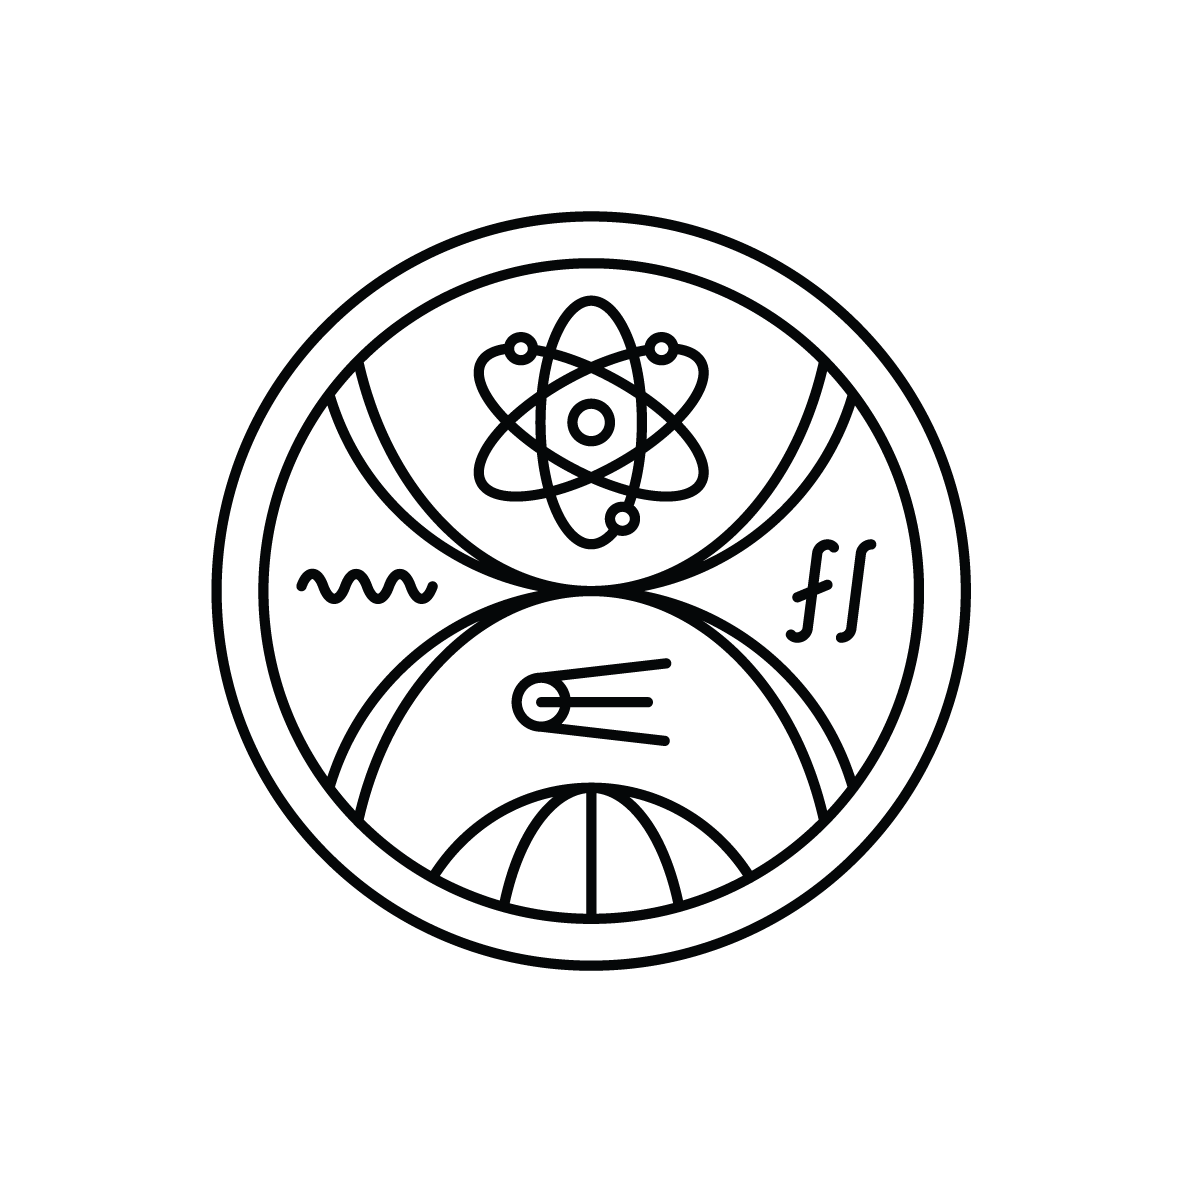
\includegraphics[width=0.4\textwidth]{images/FMFI_logo_BP}
		\label{img:logo}
	\end{center}\label{fig:figure}
\end{figure}
\begin{center}
		\textbf{\MakeUppercase{\Large\mftitle}}\\
		\mfthesistype
\end{center}
\vfill
\mfrok \hfill
\mfauthor
%\eject 
\cleardoublepage
% --- koniec obalky ----



% -------------------
% --- Titulný list
% -------------------
\thispagestyle{empty}
\noindent
\begin{minipage}{\textwidth}
    \begin{center}
        \textbf{\mfuniversity \\
        \mffaculty}
    \end{center}
\end{minipage}

\vfill
\begin{figure}[!hbt]
    \begin{center}
        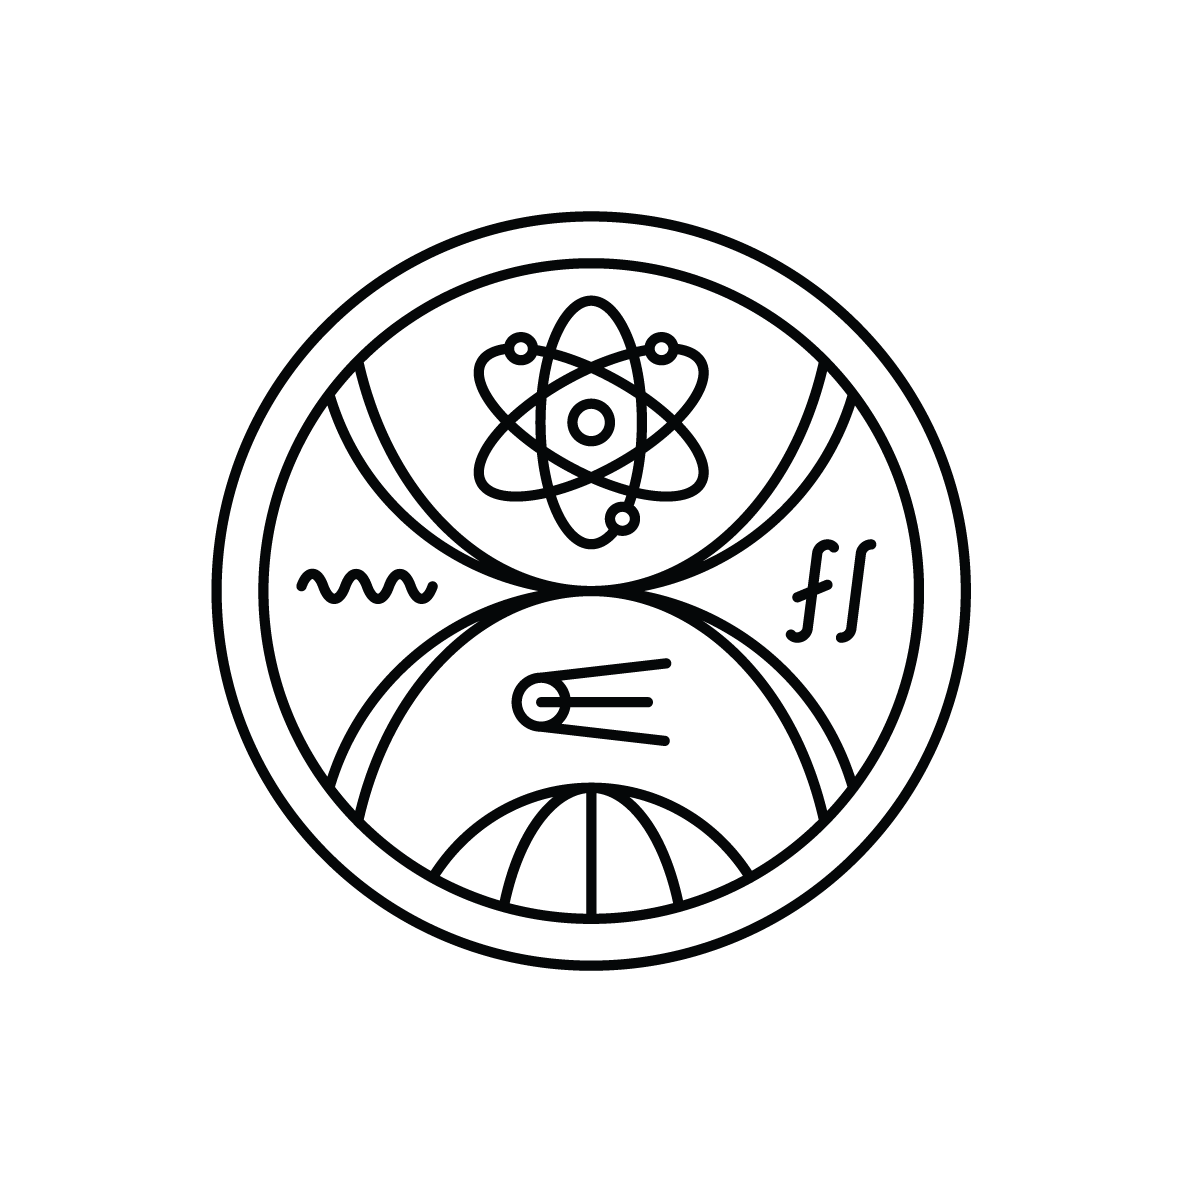
\includegraphics[width=0.4\textwidth]{images/FMFI_logo_BP}
        \label{img:logo_dark}
    \end{center}\label{fig:figure2}
\end{figure}

\begin{center}
	\textbf{\MakeUppercase{\Large\mftitle}}\\
	\mfthesistype
\end{center}
\vfill


\begin{tabular}{l l}
Study program: & \program \\
Branch of study: & \mfodbor \\
Department: & \mfpracovisko \\
Supervisor: & \mfskolitel \\
Consultant: & \mfkonzultant \\
\end{tabular}

\vfill
\noindent
\mfplacedate \hfill
\mfauthor
%\eject 
\cleardoublepage
% --- Koniec titulnej strany



% -------------------
% --- Zadanie z AIS
% -------------------
% v tlačenej verzii s podpismi zainteresovaných osôb.
% v elektronickej verzii sa zverejňuje zadanie bez podpisov
% v pracach v naglictine anglicke aj slovenske zadanie

\newpage 
\thispagestyle{empty}
\hspace{-2cm}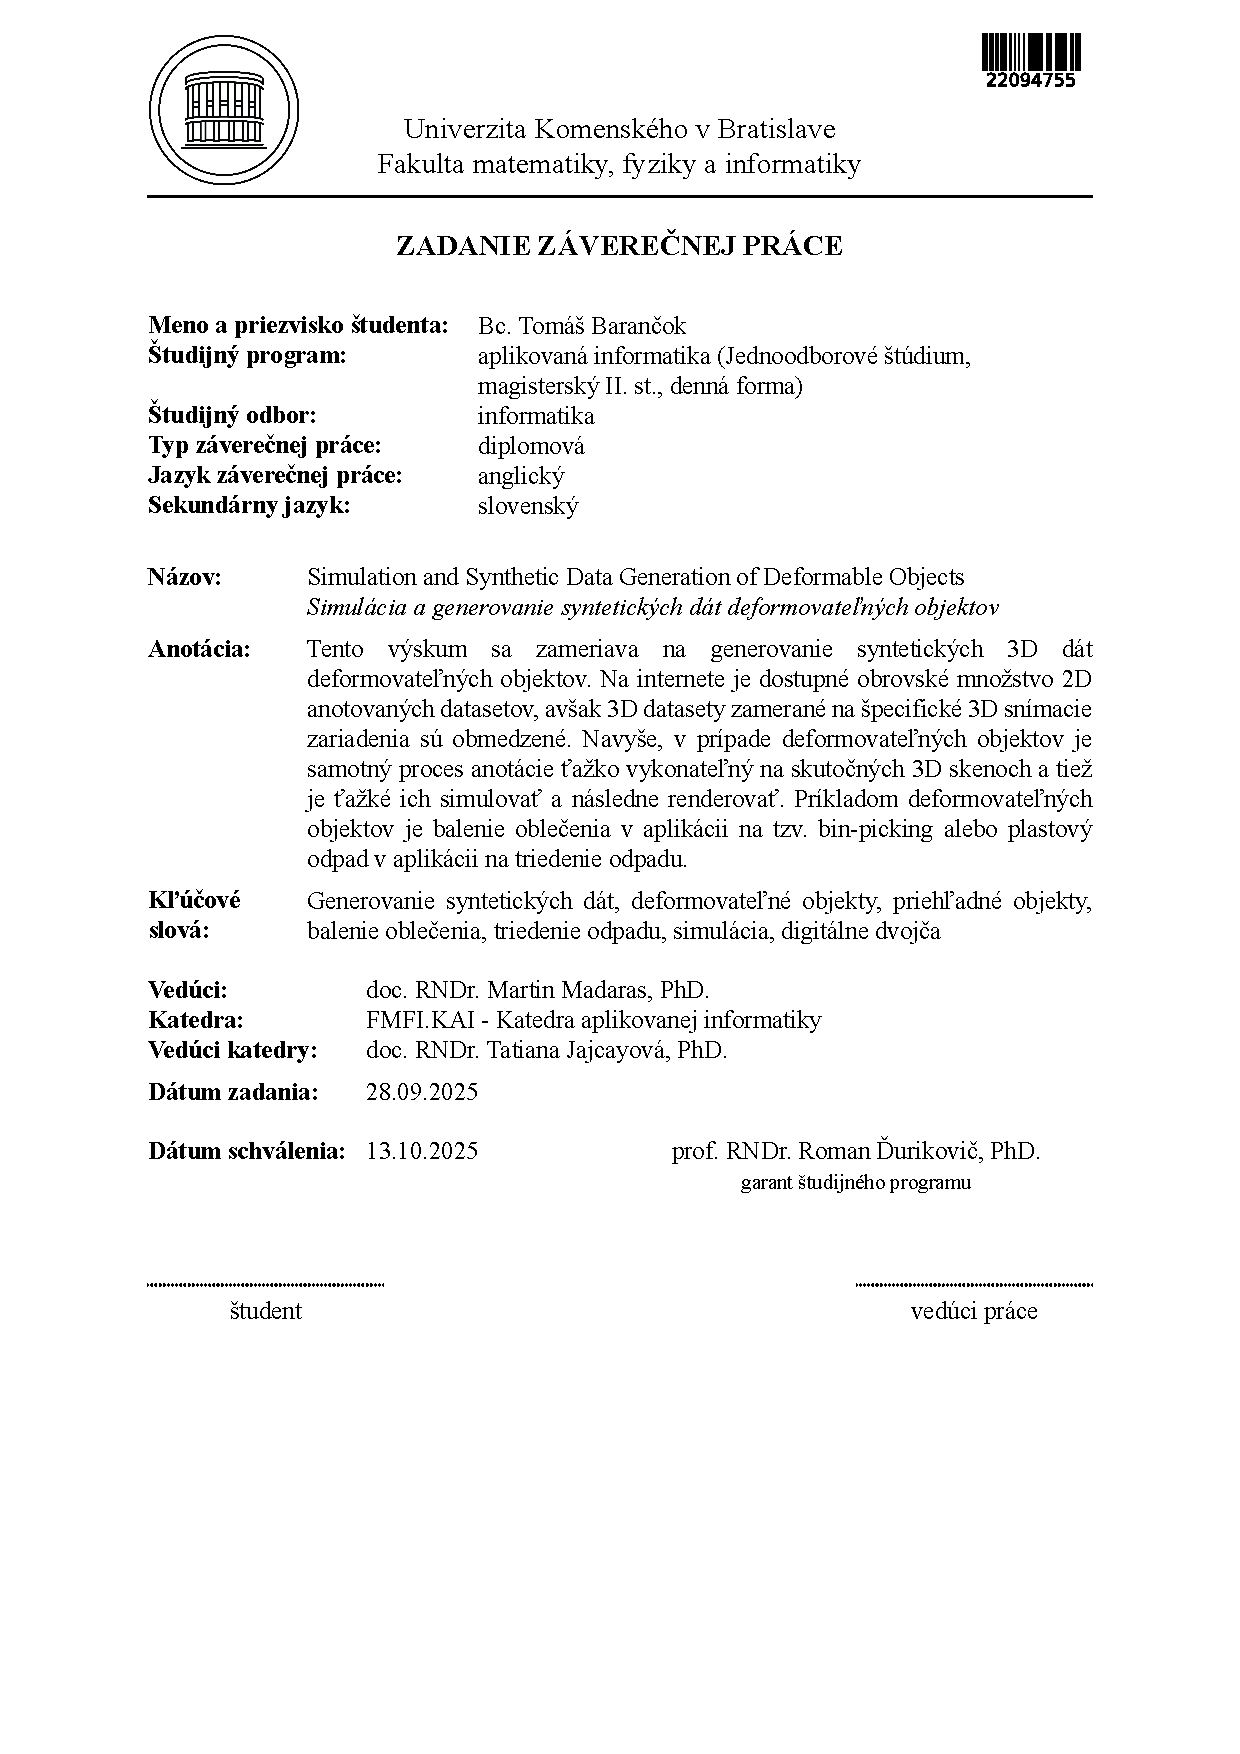
\includegraphics[page=1,width=1.1\textwidth]{zadanie-zp_204939}

\newpage
\thispagestyle{empty}
\hspace{-2cm}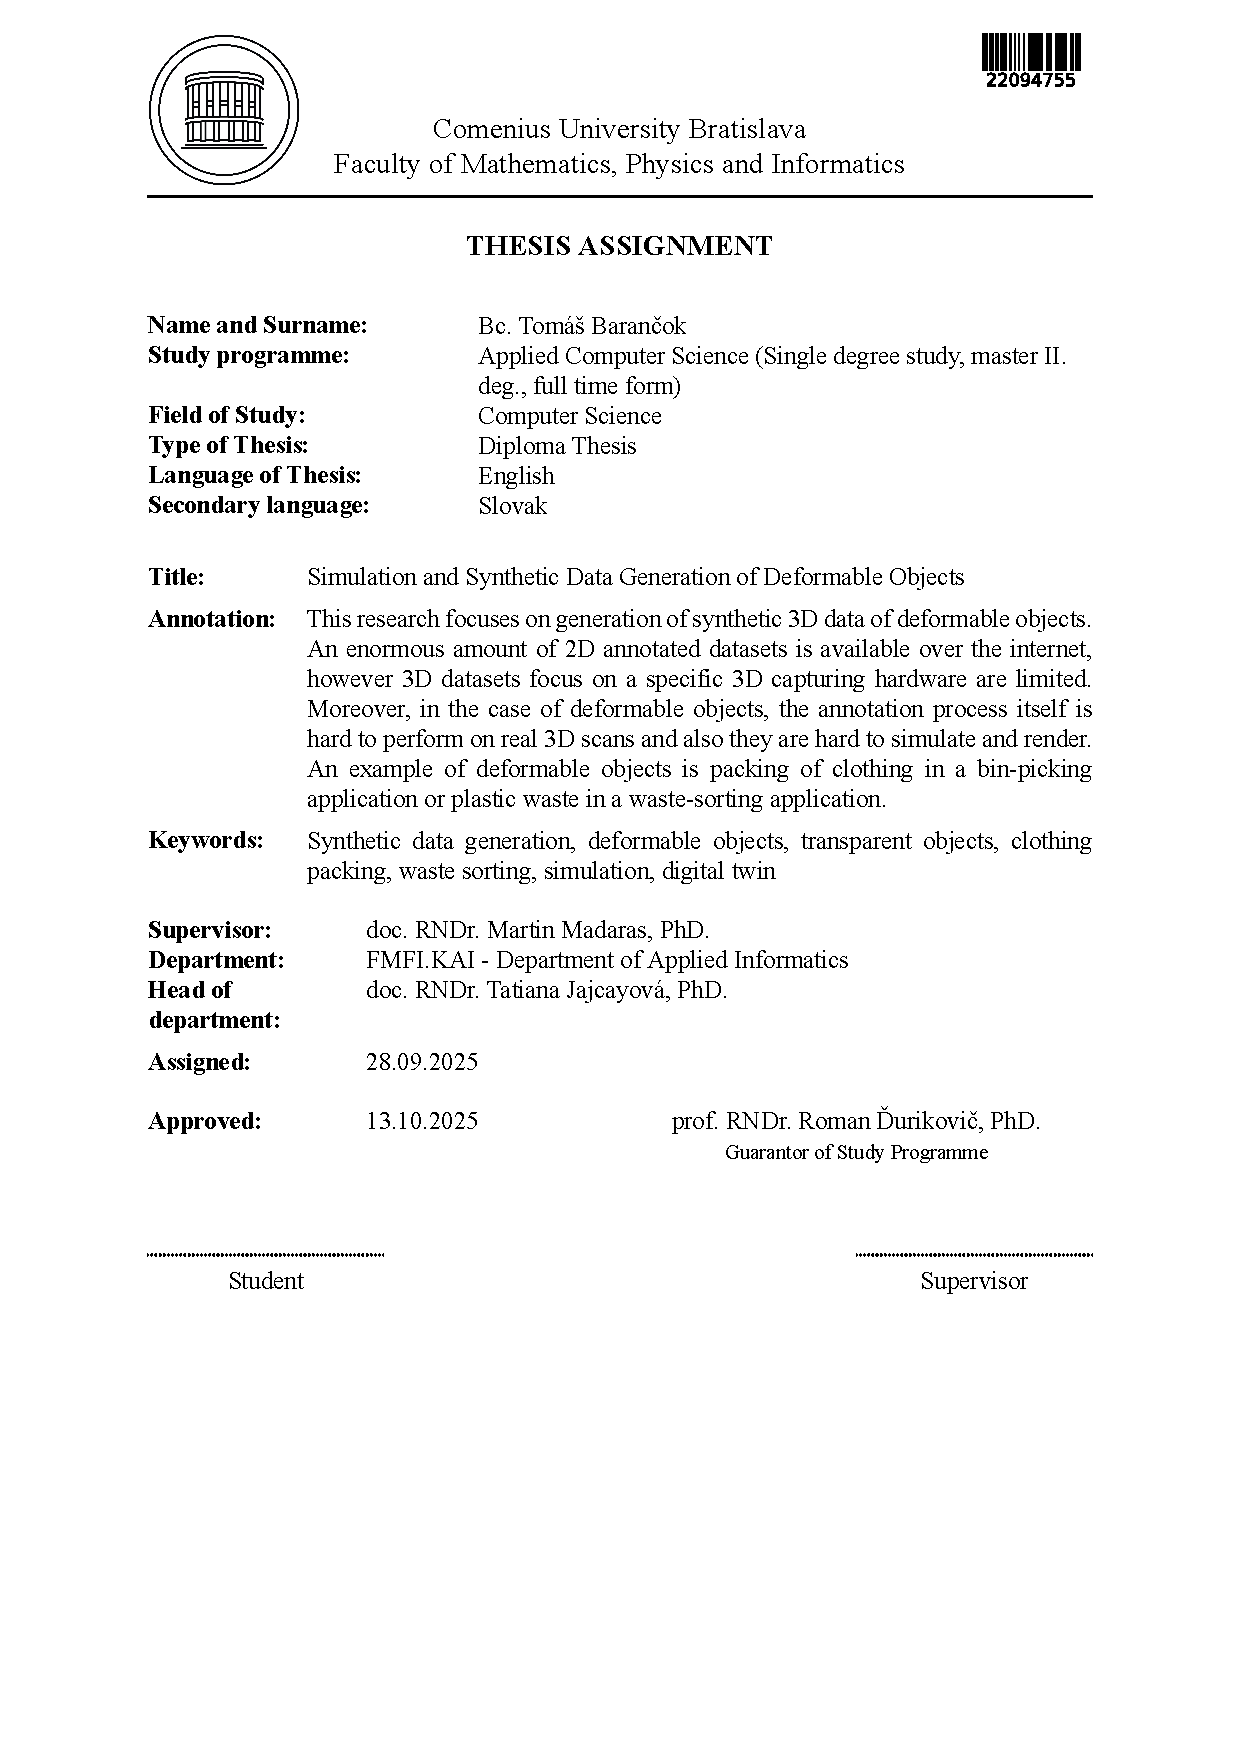
\includegraphics[page=1,width=1.1\textwidth]{zadanie-zp_204939en}

% --- Koniec zadania


% -------------------
% --- Prehlásenie
% -------------------

{~}\vspace{12cm}

\noindent
\begin{minipage}{0.25\textwidth}~\end{minipage}
\thispagestyle{empty}
\begin{minipage}{0.75\textwidth}
I hereby declare that I have written this thesis by myself, only with help of referenced literature, under the careful supervision of my thesis advisor.
\newline \newline
\end{minipage}
\vfill
~ \hfill {\hbox to 6cm{\dotfill}} \\
\mfplacedate \hfill \mfauthor
\vfill\eject \cleardoublepage
% --- koniec prehlasenia




% -------------------
% --- Poďakovanie
% -------------------
\newpage
\thispagestyle{empty}
\chapter*{Acknowledgement}\label{chap:thank_you}
Yes... TODO

\vfill\eject 
% --- koniec podakovania



% -------------------
% --- Abstrakty
% -------------------
\newpage 
\thispagestyle{empty}
\chapter*{Abstract}\label{chap:abstract_en}
\input{abstract}

\paragraph*{Keywords: Synthetic data generation, deformable objects, transparent objects, clothing
packing, waste sorting, simulation, digital twin}


\newpage 
\thispagestyle{empty}
\chapter*{Abstrakt}\label{chap:abstract_sk}
\input{abstrakt}

\paragraph*{Kľúčové slová: Generovanie syntetických dát, deformovateľné objekty, priehľadné objekty,
    balenie oblečenia, triedenie odpadu, simulácia, digitálne dvojča}


% --- koniec abstraktov


% -------------------
% --- Obsah
% -------------------
\newpage 
\tableofcontents

% ---  Koniec Obsahu


% -------------------
% --- Zoznamy tabuliek, obrázkov - nepovinne
% -------------------
\newpage 
\listoffigures
\listoftables
% ---  Koniec Zoznamov

\chapter*{Terminology}

\section*{Terms}

\begin{itemize}
    \setlength\itemsep{1px}
    \item \textbf{one} \\
    One.
    
\end{itemize}

\section*{Abbreviations}

\begin{itemize}
    \setlength\itemsep{1px}
    \item \textbf{ABB} - abbreviation.

\end{itemize}






\mainmatter

\chapter{Introduction}\label{ch:introduction}

This is our work, we do this, we do this because this and these things can be found in our work.
\chapter{Overview}\label{ch:overview}


\section{Related Works}\label{sec:related-works}
These are some works we mention.
These include for example~\cite{kibbaka} and~\cite{article}.
May include subsections.

\section{Implementation Problems}\label{sec:implementation-problems}
Unused engines, ISAAC Sim, \ldots

\chapter{Methodology}\label{ch:methodology}


\section{Blender}\label{sec:blender}

\subsection{Rendering Engine}\label{subsec:rendering-engine}

\subsection{Scripting}\label{subsec:scripting}

\subsection{Bakes}\label{subsec:bakes}

There will probably be more things, but currently I don't know.

\section{Physics Simulation}\label{sec:physics-simulation}


\section{Realisticity metrics}\label{sec:realisticity-metrics}

Subject to change.
\chapter{Implementation}\label{ch:implementation}


\section{Installation and Requirements}\label{sec:installation-and-requirements}


\section{Bottle Parametrization}\label{sec:bottle-parametrization}


\section{Material Simulation and Deformation}\label{sec:material-simulation-and-deformation}

Cloth bad, soft-body good, yap yap yap \ldots 

\section{Rendering}\label{sec:rendering}


\section{Exporting}\label{sec:exporting}
\chapter{Data Generation}\label{ch:data-generation}


\section{Scene Creation}\label{sec:scene-creation}


\section{Dataset Creation}\label{sec:dataset-creation}


\section{Dataset Testing}\label{sec:dataset-testing}
\chapter{Results}\label{ch:results}

Self-explanatory that this will contain the results.
\chapter{Conclusion}\label{ch:conclusion}

We conclude our work here.


%main content 


% -------------------
% --- Bibliografia
% -------------------

\backmatter

\nocite{*}
\bibliographystyle{plain}
\bibliography{references}

%---koniec bibliografie

\end{document}